% begin module hyperbolic-functions-applications
%todo: break this into separate slides and rename appropriately 

\begin{frame} 
Applications arise when entities such as light, velocity, electricity, radioactivity, etc. are gradually diminished.\\
A common application is to describe the shape of a hanging wire. When a heavy flexible cable (such as a telephone or power line) is suspended between two points at the same height, then it takes the shape of a curve with equation $ y=c+a\cosh(x/a) $ called a \textit{catenary}  (The Latin word \textit{catena} means ``chain.")\\
\begin{center}
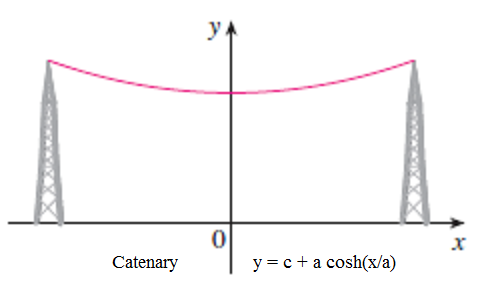
\includegraphics[width=0.35\linewidth]{../../modules/hyperbolic-functions/pictures/catenary}
\end{center}
\end{frame}

\begin{frame} 
Another application of hyperbolic functions occurs in the description of ocean waves:\\
\url{http://math.stackexchange.com/questions/123/real-world-uses-of-hyperbolic-trigonometric-functions} \\
The catenary has a corresponding surface of revolution, the \textit{catenoid}. It is the only (non-degenerate) surface of revolution that with zero mean curvature (i.e. they are minimal surfaces). This surface is the form a soap bubble (approximately) takes when it is stretched across two rings:

\begin{figure}
\centering
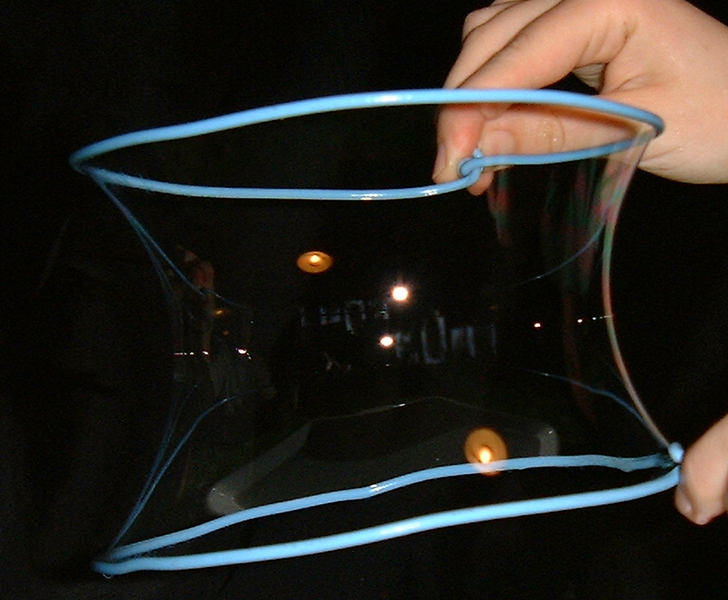
\includegraphics[width=0.5\linewidth]{../../modules/hyperbolic-functions/pictures/catenoide}
% Freely licensed : https://commons.wikimedia.org/wiki/File:Bulle_cat%C3%A9no%C3%AFde.png
%\caption{}
%\label{fig:catenoid}
\end{figure}

%The velocity of a water wave with length moving across a body of water with depth is
%modeled by the function
\end{frame}
% end module hyperbolic-functions-applications
